\documentclass[10pt,a4paper]{article}
%You comment with the modulo-sign. Before the \begin keyword you put what packages
%you want to use etc. If you want to include graphics for example you need the graphicX-package
\usepackage{graphicx}
\usepackage{amsmath}
\usepackage{float}
%You also define your title here. You create a title by putting maketitle after you have begun the document
\title{Project Plan}
\author{\begin{large}{Robotics safety}\end{large}\\\\
Olle Fridolfsson\\  Niklas Hansson\\ Patrik Hillgren\\ Benjamin Ingberg\\ Par Lundgren\\ Mattias Nilsson}
\setlength{\parindent}{0cm}	%This removes the automatic indentation
\begin{document}
\maketitle
%Latex keeps track of your sectioning automatically. To get a table of contents just put
\newpage
\tableofcontents
%To get a new page just put
\newpage
\noindent %Just makes it so that the first paragraph isn't indented
\section{Project Background}
Include something here
\section{Project Description}
Robots like Motoman are very strong compared to humans. It is therefore very important that the robot can sense when humans approach it so that it can take precautions and not hurt anyone.The goal of the project is to be able to determine the distance between the closest moving object and the robot and send a control signal to the robot depending on that information. The control signal should determine four states:

\begin{itemize}
  \item The closest moving object is outside safety zone 2 (see figure below). Objects are not in the collaborative area, the robot can work at standard motion.
  \item The closest moving object is within safety zone 2. This means that the robot motion shall be reduced since the moving object is within the collaborative area.
  \item The closest moving object is within safety zone 1. This means that the robot must stop.
  \item The closest moving object is within emergency zone. This means that the robot must perform an emergency stop, which differs from the usual stop.
\end{itemize}

\begin{figure}[H] 
  \centering
    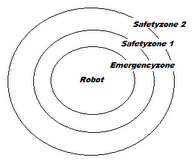
\includegraphics{safetyzones.png}
    \caption{Illustration of safetyzones}
    \label{fig:safetyzone}
\end{figure}

Determining the exact distances of the safety zones is part of the project and it is done according to the SSI ISO standard. Note that the zones is not always circular and is dependent on where the robot is positioned and in what orientation the robot is currently in.

\section{Purpose and goal}
The main purpose of this course and project is being able to solve a problem which solution requires some kind of image processing.
The project also demands independent work, one of the major goals is to make our own decisions about how we work and what we should work with. This includes defining the method used for developing and the requirements we have on our finished system.

\section{Resources}
Each group member has 240 hours at their disposal giving every sprint 60 hours of work. The physical resources includes the SIA20 Yaskawa Motoman robot, the Yaskawa DX100 controller, a few kinect sensors, the possibility to borrow laptops and a room to set up the system. 
The software will be developed using ROS Industrial.
Guidance throughout the project will be available from Johan Hedborg, Postdoc at CVL, and Richard Olsen, PhD student at IEI.

\section{Limitations}
The mapping from the kinect’s RGB camera to its depth map isn’t one to one. This might induce loss in accuracy and will not be handled unless there is time or it will have a major affect on the performance of the system. The time and knowledge of the group participants are limited. Since the project is new there are no clear guidelines available. A large part of the time will be used to get familiar and experiment with the equipment and software.

\section{Complexity}
With a possible customer in mind, a system with simple hardware is preferable in order to keep costs down. Having few components is also important to make the installation of the system as easy as possible. If the quality isn’t good enough two kinect sensors might be used instead of one. However the software should be developed such that it supports a multiple camera setup from the beginning.

\section{Project organization}
We decided that the most suitable way of working is with agile programming where the possibility to make changes is practical and easy. This is mainly because we had good experience with it before and that we are very uncertain on how the solution will look like in the end. We choose to work with the software developing method SCRUM, however in a modified way to better adjust our group and goals. The main difference with our way of working compared to traditional SCRUM is that we will not have an appointed SCRUM master or project manager. This is because we are only six members in the group and we will as much as we can work in pairs. Our way of working will be very dynamical and will contain stand up meetings at least two times a week where we go through where we are in the project and what the next step will be. We will also be working in sprints, that is working with predefined problems under 2-3 weeks and then present the so far finished product. After each sprint we will have a sprint retrospective before we start the next iteration, where we evaluate the product and the work behind it.

\section{Interested Parties}
The obvious interested parties for this project is IEI, CVL and Yaskawa. But depending on the result it can also be interesting for other companies developing robots. A good result from this project will not be dependent on the robot that is used for the development.

\section{Planning of sprints}
We will be working in sprints that will extend over 2-3 weeks. This gives us the advantage of dividing the working hours more easily and specify what they should contain. Below are a table showing a rough planning of our sprints, note that there is a possibility that sprints will extend over shorter period of time and therefore the number of sprints will increase.

\subsubsection*{Sprint 1}
\begin{itemize}
  \item Documentation
	\begin{itemize}
	\item Project Plan
	\item System Overview
	\item Design Specification
	\end{itemize}
	\item Set up
	\begin{itemize}
	\item Install ROS Industrial
	\item Connect with the robot
	\item Connect with the kinect
	\end{itemize}
\end{itemize}
\subsubsection*{Sprint 2}
\begin{itemize}
\item Test
\begin{itemize}
\item Process data from robot controller to obtain 3D coordinates
\item Control robot
\item Try different setups of cameras and robot
\end{itemize}
\end{itemize}
\subsubsection*{Sprint 3}
\begin{itemize}
\item Coding
\begin{itemize}
\item Identify robot from other objects in the image
\item Link robot depth information to the data containing the position of the robot
\item Determine distance from the robot to all other moving objects in the scene
\end{itemize}
\end{itemize}
\subsubsection*{Sprint 4}
\begin{itemize}
\item Refining
\begin{itemize}
\item Speedup and Improvements
\item Documentation
\item Evaluation
\item Bug fixing
\end{itemize}
\end{itemize}

\end{document}